\section{Zielspezifikationen}

Bevor mit der Entwicklung begonnen wurde, mussten Ziele aufgestellt werden.

\begin{itemize}
    \item Das Licht muss hell genug leuchten, um das Aufleuchten bei Tageslicht zu erkennen.
    \item Das System muss Batteriebetrieben sein.
    \item Die Platine soll energieeffizient sein, damit das Fahrradlicht lange genug haltet.
\end{itemize}


\section{Blockdiagramm}

Das Blockdiagramm in Abbildung \ref{fig:blockdiagramm} veranschaulicht, wie die einzelnen Komponenten des Fahrradlichts miteinander interagieren.

\begin{figure}[H]
    \centering
    \includegraphics[width=0.7\textwidth]{resources/Block Diagrams/Overview.png}
    \caption{Funktionsblockdiagramm}
    \label{fig:blockdiagramm}
\end{figure}

\noindent Die Batterie versorgt die verschiedenen Teile der Schaltung: 
Einerseits werden die LEDs über ein Step-Up-Modul mit $5\,\text{V}$ betrieben, 
andererseits erhalten die digitalen Komponenten eine Versorgungsspannung von $3{,}3\,\text{V}$ vom Low-Dropout-Spannungsregler (LDO). 
Der Mikrocontroller misst über eine Messschaltung (Abbildung \ref{fig:batteriemessung}) die Batteriespannung. 
Die Batterie wird über einen Ladechip sowie eine Batterieschutzschaltung geladen. 
Der Ladechip informiert den Mikrocontroller zudem, ob die Batterie aktuell geladen wird oder bereits vollständig geladen ist. 
Darüber hinaus übernimmt der Mikrocontroller die Kommunikation sowohl mit dem Beschleunigungssensor als auch mit den LEDs und koordiniert deren Steuerung.



\section{Komponentenwahl}

\subsection{Mikrocontroller}
Angesichts der Anforderungen dieses Projekts musste der Mikrocontroller nichts Besonderes sein. Ziel war es, einen stromsparenden Chip zu finden, der I$^2$C unterstützt. Außerdem sollte er günstig und weit verbreitet verfügbar sein. Aufgrund guter Erfahrung bei vorherigen Projekten wurde zu Beginn der ATTiny1616 unter Betracht bezogen. Dieser hat ein sehr kleines QFN-20 Package und ist ein moderner Microchip Microcontroller.

\subsection{Beschleunigungssensor}
Der Beschleunigungssensor wird zur Bremserkennung verwendet. Hierfür gab es viele Optionen, darunter auch der sehr populäre und ausführlich dokumentierte MPU6050. Da jedoch großer Wert auf die Batterielaufzeit gelegt wurde, fiel die Wahl aufgrund seines niedrigen Stromverbrauchs auf den \textbf{LIS3DHTR} von STMicroelectronics.
\subsection{LEDs}
Für die LEDs wurden einige Optionen in Betracht gezogen:

% TODO: Change this to a list?
\subsubsection{High Power LEDs}
HIGH Power LEDs leuchten erstaunlich hell, haben aber den Nachteil das sie gekühlt werden müssen. Für eine LED dieses Typs hätte vermutlich ein passiver Kühlkörper oder eine Kupferfläche auf der Leiterplatte gereicht, jedoch hätte dies extra Platz im Gehäuse verbraucht.

\subsubsection{Bedrahtete 5mm LEDs}
Diese kann man als herkömmliche LEDs bezeichnen. Ihre THT-Bauform bedeutet jedoch, dass sie mehr Platz auf der Platine beanspruchen würden. Außerdem gab es immer wieder Diskussionen, ob diese Hell genug sein würden. Unterumständen hätten sie auch einen eigenen \textbf{Constant-Current Driver} benötigt. 
% TODO: Return Paths? 
\subsubsection{WS2812}
Für dieses Projekt wurden WS2812-RGB-LEDs gewählt. Sie werden häufig in RGB-Streifen eingesetzt und zeichnen sich durch ihre hervorragende Helligkeit aus. Außerdem liegen im Team bereits Erfahrungen mit ihrer Ansteuerung vor, und sie ermöglichen einfache Animationen, z.B. Ladeanimationen.



\subsection{Batterie}

Bei der Auswahl der Batterie wurde ein Kompromiss zwischen Typ, Baugröße und Kapazität angestrebt. 
Daher fiel die Wahl auf einen LiPo-Akku mit einer Kapazität von $1500\,\text{mAh}$. 
Diese Kapazität ermöglicht eine ausreichende Laufzeit, ohne dass die Abmessungen die Größe der Leiterplatte wesentlich überschreiten.


\subsection{Ladechip}
Der Ladechip ist der TP4056. Der größte Grund warum sich dafür entschieden wurde, sind die Resourcen die man Online findet und die Erfahrung die das Team mit diesen Komponenten bereits hat. Er besitzt einen einstellbaren Ladestrom von bis zu 1A und ist einfach zu beschalten. 



\section{Firmware Architektur}
%TODO: Modi des Fahrradlicht (Sleep etc)

\section{PCB Design}
\subsection{Schaltpläne}
% TODO: Explain each Schematic Block 

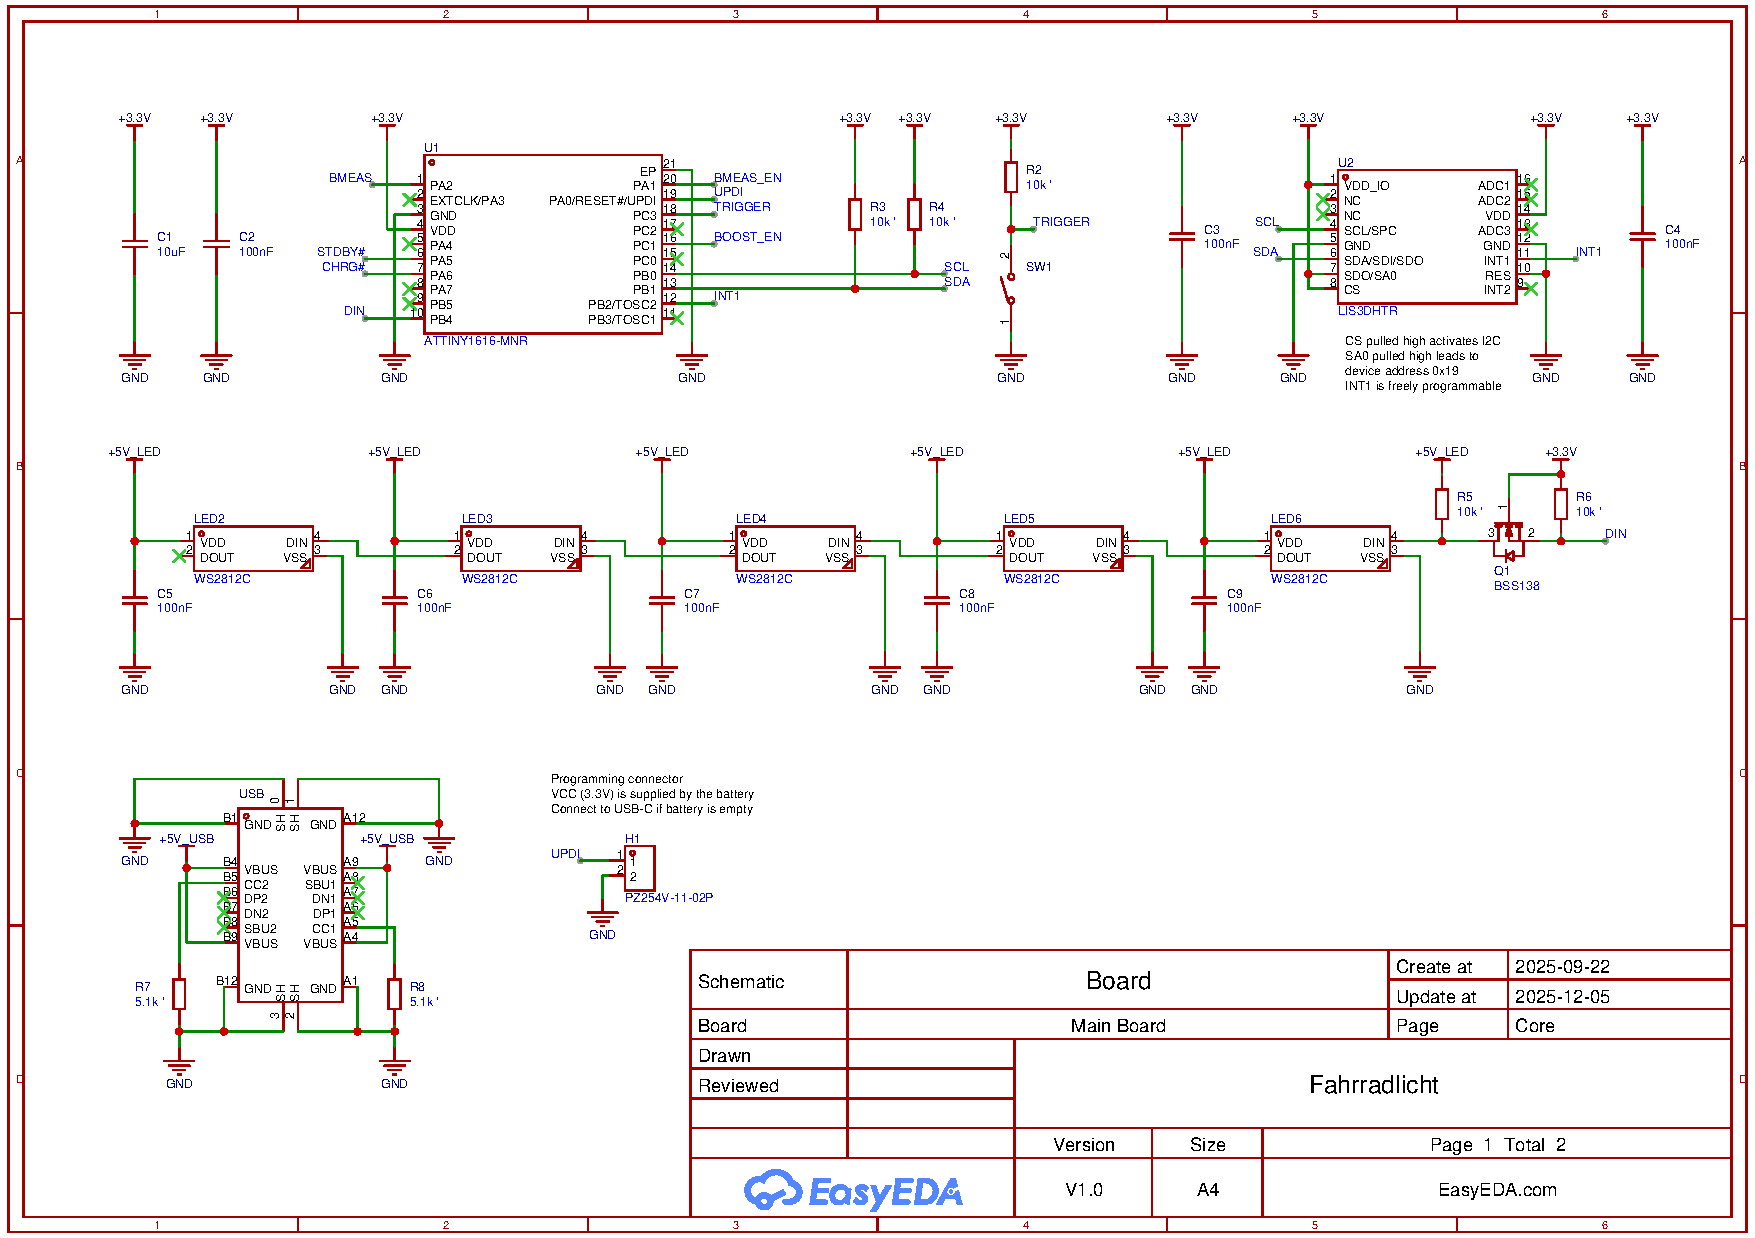
\includepdf[angle=90]{resources/Schematics/Page1.pdf}
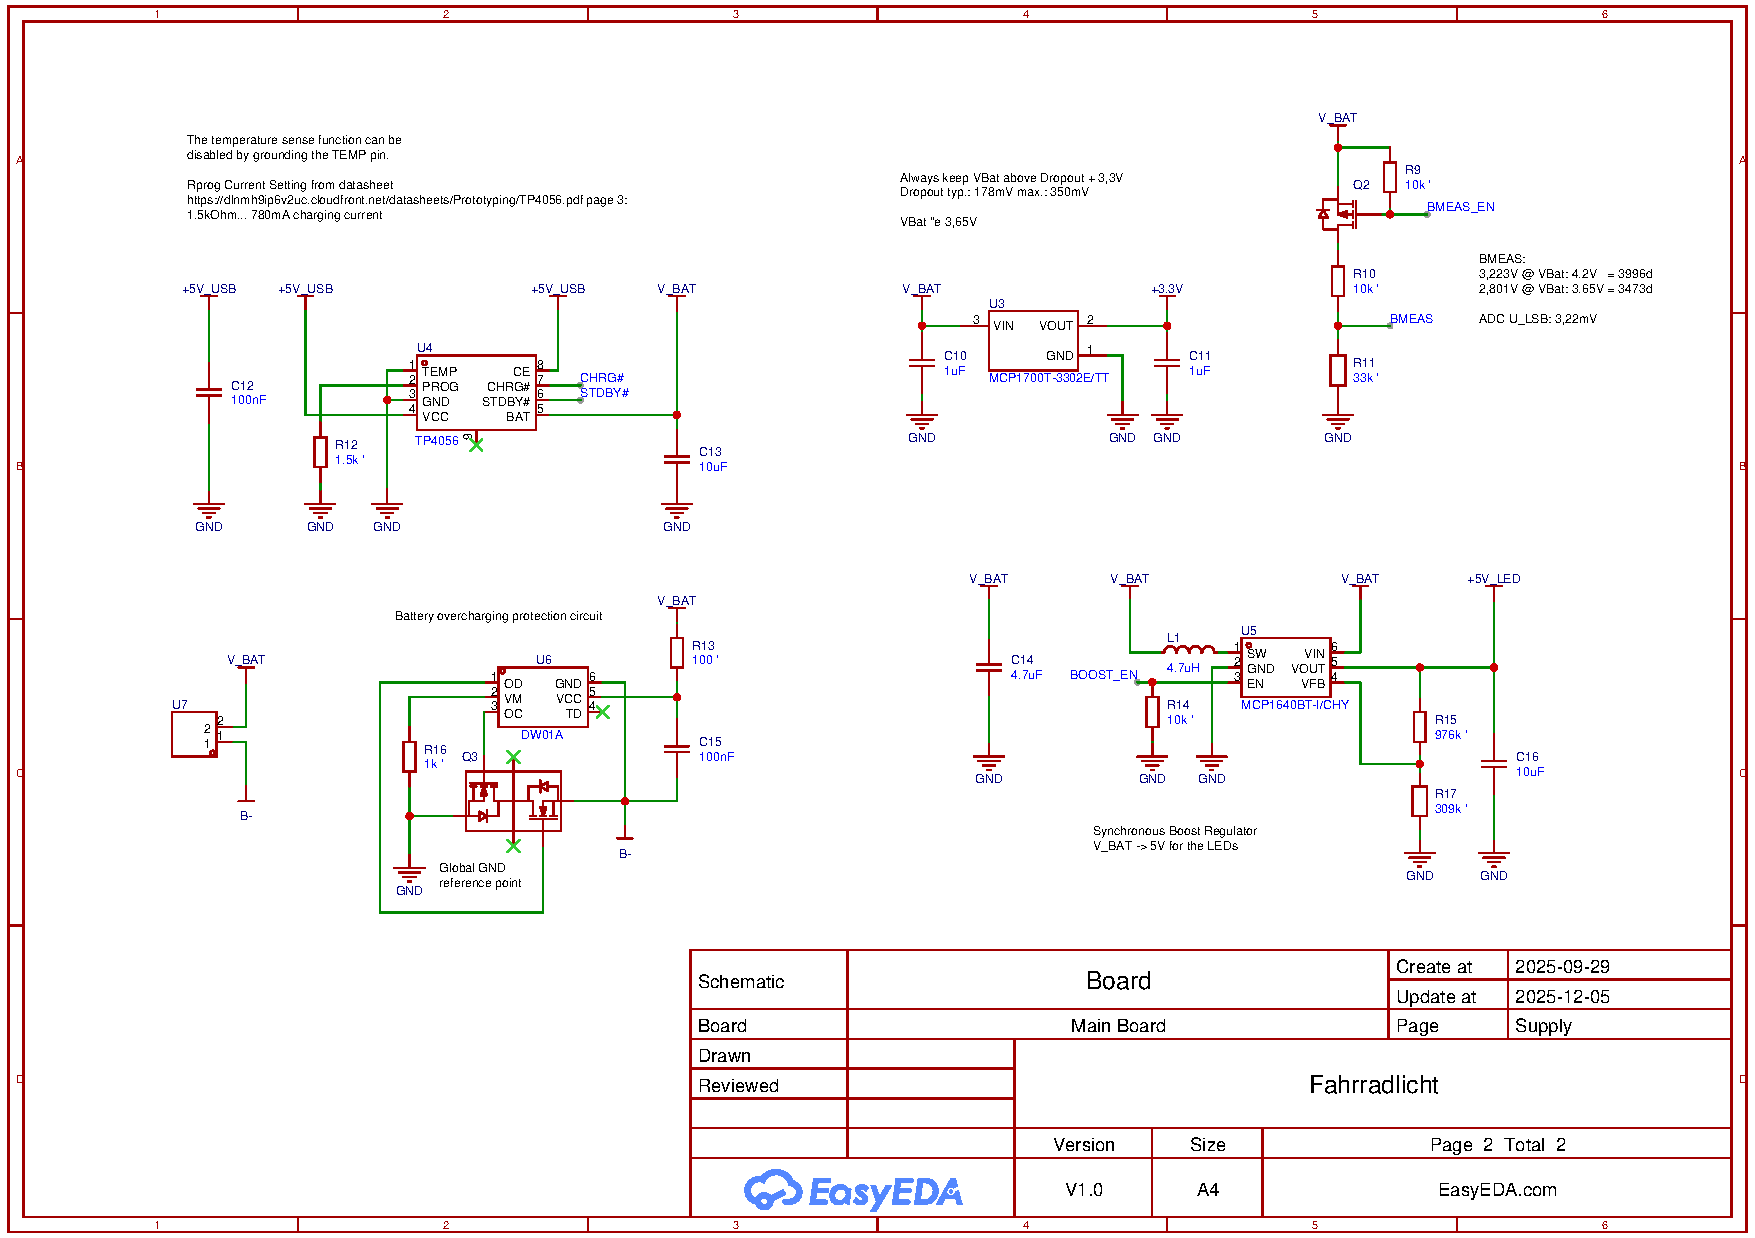
\includepdf[angle=90]{resources/Schematics/Page2.pdf}

\subsection{Schaltblöcke}

Der ATTiny1616 Mikrocontroller ist, aufgrund seiner typischen Anwendungen einfach zu beschalten. Zur grundlegenden Operation werden hauptsächlich die Versorgungsleitungen ($V_{CC}$ und $GND$) benötigt. Der Chip wird über dass UDPI (Unified Program and Debug Interface) programmiert, welches sich auf jeden der neueren Chips der ATTiny-Serie befinden. 

% TODO: Schematic of turning a standard RX TX Adapter into a UDPI Programmer

\subsubsection{Mikrocontroller}
$C1$ und $C2$ sind Stützkondensatoren um glätten der Versorgung. $R3$ und $R4$ sind Pull Up Widerstände, um den $I2C$-Bus betreiben zu können. Es gibt auch einen Button \texttt{SW1} um das Fahrradlicht bedienen zu können.
\begin{figure}[H]
    \centering
    \includegraphics[width=\textwidth]{resources/Schematics/MCU.png}
    \caption{Mikrocontroller}
\end{figure}

\subsubsection{Beschleunigungssensor}
Der LIS3DHTR muss über seine Pins konfiguriert werden. Er kann sowohl über I2C als auch über SPI betrieben werden. In diesem Projekt wurde er auf I2C konfiguriert, weshalb der Pin \texttt{CS} auf HIGH gesetzt wurde. Außerdem dient dieser Pin dazu, die I2C-Adresse festzulegen. Die ADCs werden nicht verwendet. Die Kondensatoren $C3$ und $C4$ sind laut der Application Note mit $100\,\text{nF}$ bestückt. Der \texttt{INT1}-Pin dient als Interrupt und wird zum Mikrocontroller geführt. Dies wurde als Stromsparmaßnahme getan.

\begin{figure}[H]
    \centering
    \includegraphics[width=0.7\textwidth]{resources/Schematics/Sensor.png}
    \caption{Beschleunigungssensor im Schaltplan}
\end{figure}


\subsubsection{LEDS}
Laut Datenblatt soll jede WS2812-LED mit einem Stützkondensator mit einem Wert von $100\,\text{nF}$ beschaltet werden. 
Da diese adressierbaren LEDs mit einer $5\,\text{V}$-Logik arbeiten, wurde mithilfe eines \texttt{BSS138}-MOSFETs ein Logikpegelwandler realisiert, der das $3{,}3\,\text{V}$-Signal der MCU auf $5\,\text{V}$ umsetzt. 
Obwohl ein $3{,}3\,\text{V}$-Signal am Datenpin unter Umständen ebenfalls funktioniert hätte, wurde diese Lösung gewählt, um die Funktionalität zu gewährleisten und mögliche Risiken zu vermeiden.

% TODO: Add citation to sparkfun site for this level shfiter

\begin{figure}[H]
    \centering
    \includegraphics[width=\textwidth]{resources/Schematics/LEDs.png}
    \caption{LEDs im Schaltplan}
\end{figure}

\subsubsection{Anschlüsse}
Für das Hochladen der Firmware wurde UDPI verwendet. Dafür wurden die Pins \texttt{GND} und \texttt{UDPI} auf zwei Pins herausgeführt. 
$V_{CC}$ wurde ausgelassen, um Platz auf der Leiterplatte zu sparen. 

\begin{figure}[H]
    \centering
    \includegraphics[width=0.7\textwidth]{resources/Schematics/UDPI_Pins.png}
    \caption{UDPI Stecker im Schaltplan}
\end{figure}

\noindent Geladen wird das Fahrradlicht über eine USB-C Buchse. Aufgrund der USB-PD Spezifikationen müssen die Leitungen \texttt{CC1} und \texttt{CC2} auf GND über $5,1k\Omega$ Widerstände gezogen werden, da sonst nicht die richtige Spannung vom Netzteil angefragt werden kann.

\begin{figure}[H]
    \centering
    \includegraphics[width=0.7\textwidth]{resources/Schematics/USBC.png}
    \caption{USB-C im Schematic}
\end{figure}

\subsubsection{Ladeschaltung}
Die Application Note im Datenblatt hat sich als genügend bewiesen, obwohl es viele Resourcen zu dem TP4056 Chip online gibt. Stützkondensatoren von $100nF$ und $1\mu F$ stabiliseren die Aus- und Eingangsspannungen. Die Open-Drain Pins $CHRG$ und $STDBY$ geben aus, ob die Batterie ladet bzw. voll ist. Der Ladestrom $I_{BAT}$ wird mit einen Widerstand $R_{PROG}$ (hier R12) am \texttt{PROG}-Pin eingestellt. Die Berechnung ist wie folgt: 

\begin{align}
    V_{PROG} &= 1V \\
    I_{BAT} &= \frac{V_{PROG}}{R_{PROG}} \times 1200 \\
    R_{PROG} &= \frac{V_{PROG}}{I_{BAT}} \times 1200 \\
    R_{PROG} &= \frac{1\text{V}}{800\text{mA}} \times 1200 \\
    R_{PROG} &= 1500\Omega
\end{align}

\begin{figure}[H]
    \centering
    \includegraphics[width=0.7\textwidth]{resources/Schematics/Charging_Circuit.png}
    \caption{Ladeschaltung im Schaltplan}
\end{figure}

\subsubsection{Überladeschutz}
Der DW01A ist ein Schutz-IC für einzelne Lithium-Ionen- oder Lithium-Polymer-Zellen. Er überwacht die Zellspannung und schützt die Batterie vor Überladung, Tiefentladung sowie Überstrom. Bei Überschreitung der Grenzwerte schaltet der DW01A die Batterie über externe MOSFETs ab, um Schäden zu vermeiden und die Lebensdauer der Zelle zu erhöhen. Typischerweise wird er zusammen mit zwei externen MOSFETs in Schutzschaltungen für Akkupacks eingesetzt.
% TODO: No idea what it actually does 💀

\begin{figure}[H]
    \centering
    \includegraphics[width=0.7\textwidth]{resources/Schematics/Overcharging_Circuit.png}
    \caption{Überladeschutz im Schaltplan}
\end{figure}

\subsubsection{Boost-Converter}

Der \textbf{MCP1640} ist eine ausgezeichnete Wahl für dieses Projekt, da er einfach zu beschalten ist und wenig Strom im ausschaltenen Zustand verbraucht. 
Die Eingangsspannung kann variabel sein, wie es bei LiPo-Akkus typischerweise vorkommt, und dennoch hält er die Ausgangsspannung konstant. 
Die Schaltung aus der Application Note konnte direkt in den Schaltplan übernommen werden, wobei der Spannungsteiler aus den Widerständen $R15$ und $R17$ die Ausgangsspannung festlegt.

\begin{figure}[H]
    \centering
    \includegraphics[width=0.7\textwidth]{resources/Schematics/Boost.png}
    \caption{Boost-Converter im Schaltplan}
\end{figure}

\noindent Für Stromersparnisse wird der ENABLE-Pin des Boost-Converters vom Mikrocontroller gesteuert, wodurch die Schaltung bei Nichtgebrauch deaktiviert und der Energieverbrauch minimiert wird. 
\subsubsection{Batterieladestandsmessung}

Da die Batteriespannung Werte über dem Maximum des ADCs des Mikrocontrollers erreichen kann, wird ein Spannungsteiler verwendet, um ein geeignetes Signal zu erzeugen. 
Ein Nachteil dieser Lösung ist jedoch, dass konstant ein Strom fließt, der die Batterie entladen würde. 
Deshalb wird ein MOSFET eingesetzt, der nur durchschaltet, wenn eine Batteriemessung durchgeführt werden soll. 
Die Messung des Batterieladestands kann zudem nur sporadisch erfolgen, da sich dieser Parameter nur über größere Zeiträume verändert.

\begin{figure}[H]
    \centering
    \includegraphics[width=0.7\textwidth]{resources/Schematics/Battery_Measurement.png}
    \caption{Batteriemessungsschaltung}
    \label{fig:batteriemessung}
\end{figure}


\subsubsection{Spannungsregelung mit LDO}
Für die Versorgung des Mikrocontrollers und der Sensoren werden $3,3\,\text{V}$ benötigt. Hier kommt ein LDO-Spannungsregler zum Einsatz. 
Im Gegensatz zu herkömmlichen Spannungsreglern ist die Drop-Out-Spannung bei LDOs sehr gering, oft im Millivoltbereich. 
Dies bietet eine einfache und kostengünstige Möglichkeit, die gewünschte Spannung zu erzeugen. 
Zwar hätte man sich an der Schaltung des Boost-Converters orientieren können, jedoch erreicht dieser weder die Simplizität noch die Energieeinsparung eines LDOs.

\begin{figure}[H]
    \centering
    \includegraphics[width=0.7\textwidth]{resources/Schematics/Voltage_Regulator.png}
    \caption{Spannungsregelung mit LDO}
\end{figure}


\subsection{Layout}

Das Layout des Boards musste mehrere Anforderungen erfüllen. Es sollte professionell gestaltet werden und GND- sowie Versorgungsflächen enthalten. 
Zudem sollten mindestens zwei Stellen für Befestigungslöcher freigehalten werden. Die LEDs sowie der Taster sollten zentriert auf dem Board platziert werden. Sowohl der JST-Stecker als auch der USB-C-Anschluss wurden strategisch positioniert, um die Integration in das Gehäusedesign zu erleichtern.


\subsubsection{Kondensatoren}

Bereits beim Platzieren der Bauteile wurde darauf geachtet, die Stützkondensatoren möglichst nahe an den jeweiligen Versorgungspins zu positionieren. Dies dient dazu, Störfrequenzen sowie Spannungsschwankungen effektiv zu reduzieren. In Abbildung \ref{fig:kondensator_bei_versorgung} sieht man, dass der Kondensator \texttt{C8} nahe des Versorgungspins der \texttt{LED5} platziert wurde.

\begin{figure}[H]
    \centering
    \includegraphics[width=0.3\textwidth]{resources/Board/Layout/Capacitor_close_to_supply.png}
    \caption{Kondensator bei Versorgungspins}
    \label{fig:kondensator_bei_versorgung}
\end{figure}

\subsubsection{GND-Flächen}

GND-Flächen sind in professionellen Leiterplattendesigns weit verbreitet und bieten mehrere Vorteile. 
Zum einen ermöglichen sie einen Rückstrompfad mit niedriger Impedanz, was die elektrische Stabilität verbessert. 
Zum anderen vereinfachen sie die Leiterbahnführung erheblich: Traces müssen nicht mehr jeden Punkt direkt verbinden, sondern können über ein Via auf die andere Seite der Platine geführt werden. 
Dies reduziert den Routing-Aufwand und trägt zu einem saubereren, zuverlässigeren Layout bei.

\subsubsection{Stitching Vias}
% TODO: Put it under GND-Flächen?

\begin{figure}[H]
    \centering
    \includegraphics[width=0.3\textwidth]{resources/Board/Layout/Stitching Vias.png}
    \caption{Stitching Vias}
\end{figure}

\subsubsection{Power-Planes}
Power-Planes, auch Versorgungsflächen genannt, bieten mehrere Vorteile. Durch die großflächige Versorgung fließt der Strom nicht durch enge Leiterbahnen, wodurch Wärmeentwicklung und Spannungsabfall reduziert werden. 
Außerdem verringern große Flächen die Induktivität im Vergleich zu schmalen Traces, was insbesondere bei Mikrocontrollern zu einer stabileren Versorgung beiträgt. In Kombination mit den GND-Flächen wirken die Power-Planes wie ein großflächiger Kondensator, der elektromagnetische Störungen filtert und somit eine saubere Versorgung sicherstellt.

% TODO: The sizes are hacked, maybe just insert the images afterwards into the PDF?

\begin{figure}[H]
    \centering
    \includegraphics[width=0.4\textwidth]{resources/Board/Layout/Top.png}
    \caption{Top layer layout}
\end{figure}

\begin{figure}[H]
    \centering
    \includegraphics[width=0.4\textwidth]{resources/Board/Layout/Bottom.png}
    \caption{Bottom layer layout}
\end{figure}

%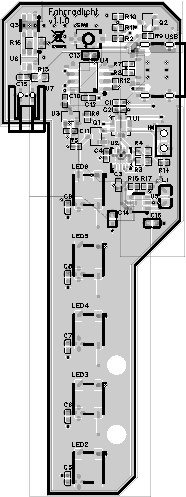
\includepdf[pages=1-2]{resources/Board/Layout/PCB.pdf}


\subsection{BOM}

% i hacked the table sizes and fuck you im proud of it
% please fix it
\begin{table}[H]
    \centering
    \begin{tabularx}{\textwidth}{|l|>{\raggedright\arraybackslash}X|>{\raggedright\arraybackslash}X|l|l|}
    \hline
        \textbf{Qty} & \textbf{Comment} & \textbf{Designator} & \textbf{Supplier Part} & \textbf{JLCPCB Price} \\ \hline
        1 & 10uF & C1 & C15525 & 0.0008 \\ \hline
        10 & 100nF & C2,C3,C4,C5,C6,C7,C8,C9,C12,C15 & C1525 & 0.0002 \\ \hline
        2 & 1uF & C10,C11 & C52923 & 0.0005 \\ \hline
        2 & 10uF & C13,C16 & C19702 & 0.001 \\ \hline
        1 & 4.7uF & C14 & C19666 & 0.0015 \\ \hline
        1 & PZ254V-11-02P & H1 & C492401 & 0.0018 \\ \hline
        1 & 4.7uH & L1 & C395016 & 0.0036 \\ \hline
        5 & WS2812C & LED2,LED3,LED4,LED5,LED6 & C114587 & 0.0145 \\ \hline
        1 & BSS138 & Q1 & C18212695 & 0.0029 \\ \hline
        1 & IRLML6402TRPBF & Q2 & C2593 & 0.0164 \\ \hline
        1 & FS8205A & Q3 & C908265 & 0.01 \\ \hline
        6 & 10k & R2,R5,R6,R9,R10,R14 & C25744 & 0.0002 \\ \hline
        2 & 10k & R3,R4 & C25804 & 0.0002 \\ \hline
        2 & 5.1k & R7,R8 & C25905 & 0.0002 \\ \hline
        1 & 33k & R11 & C25779 & 0.0002 \\ \hline
        1 & 1.5k & R12 & C25867 & 0.0002 \\ \hline
        1 & 100 & R13 & C22775 & 0.0002 \\ \hline
        1 & 976k & R15 & C25802 & 0.0001 \\ \hline
        1 & 1k & R16 & C17513 & 0.0004 \\ \hline
        1 & 309k & R17 & C5713270 & 0.0001 \\ \hline
        1 & TS-1088-AR02016 & SW1 & C720477 & 0.0065 \\ \hline
        1 & ATTINY1616-MNR & U1 & C507118 & 0.1323 \\ \hline
        1 & LIS3DHTR & U2 & C15134 & 0.111 \\ \hline
        1 & MCP1700T-3302E/TT & U3 & C39051 & 0.0524 \\ \hline
        1 & TP4056 & U4 & C42422118 & 0.007 \\ \hline
        1 & MCP1640BT-I/CHY & U5 & C478087 & 0.1204 \\ \hline
        1 & DW01A & U6 & C351410 & 0.0061 \\ \hline
        1 & S2B-PH-K-S(LF)(SN) & U7 & C173752 & 0.0052 \\ \hline
        1 & TYPE-C-31-M-12 & USB & C165948 & 0.0259 \\ \hline
    \end{tabularx}
\end{table}

Der Preis mit Bestückungsservice und Versandkosten lief auf JLCPCB auf PREIS aus. % TODO, Preis


\section{3D Design}
Das Gehäuse wurde in Autodesk Fusion konzipiert. 
\subsection{Vorraussetzungen}

\begin{itemize}
    \item Das Gehäuse soll kompakt gehalten werden.
    \item Es soll möglichst einfach zu montieren sein.
    \item Es darf kein Wasser in das Gehäuseinnere eintreten.
    \item Ein Ausschnitt für den Ladeport muss vorhanden sein.
    \item Es soll in 3D-Druck, bevorzugt FDM-Druck gefertigt werden. 
\end{itemize}


\subsection{Gehäuse}

\begin{figure}[H]
    \centering
    \begin{subfigure}{0.48\textwidth}
        \centering
        \includegraphics[width=\textwidth]{resources/CAD/Design-3kx3k.png}
        \caption{Ansicht 1}
    \end{subfigure}\hfill
    \begin{subfigure}{0.48\textwidth}
        \centering
        \includegraphics[width=\textwidth]{resources/CAD/Design-3kx3k-2.png}
        \caption{Ansicht 2}
    \end{subfigure}
    \caption{Gehäuse des Fahrradlichts}
    \label{fig:cases}
\end{figure}

Wie in Abbildung \ref{fig:cases} zu erkennen ist, wurde für das Gehäusedesign eine organische Form gewählt. 
Ein boxartiges Design sollte vermieden werden. 
Dies führte jedoch dazu, dass die Fertigung mittels FDM-Druck erschwert wird; 
daher wurde auch der SLA-Druck in Betracht gezogen.

% TODO: FDM vs SLA?

% TODO: Rewrite this shit 😭
Um das Gehäuse wasserdicht auszuführen, wurde der Einsatz verschiedener Materialien in Betracht gezogen. 
Es ist vorgesehen, eine Dichtung aus TPU zu fertigen, die bei der Montage in die Innenwände des Gehäuses eingesetzt wird. 
Zusätzlich soll der USB-C-Port durch einen wasserdichten Stöpsel gegen das Eindringen von Wasser geschützt werden.


Für die Befestigung am Fahrrad ist die Verwendung eines Gummirings vorgesehen. 
Dieser kann entweder als Standardbauteil zugekauft oder alternativ ebenfalls aus TPU gefertigt werden.

% TODO: Render of pole 

Der LiPo-Akku ist hinter der Leiterplatte im Gehäuse positioniert (siehe Abbildung \ref{fig:batterie_im_gehaeuse}). 
Daraus ergab sich die besondere Form der Leiterplatte, die eine einfache Führung des Akkukabels in den hinteren Teil des Gehäuses ermöglicht.

\begin{figure}[H]
    \centering

    \begin{subfigure}[b]{0.35\textwidth}
        \centering
        \includegraphics[width=\textwidth]{resources/CAD/Shell with battery.png}
        \caption{Batterie im Gehäuse}
        \label{fig:batterie_im_gehaeuse}
    \end{subfigure}
    \hfill
    \begin{subfigure}[b]{0.35\textwidth}
        \centering
        \includegraphics[width=\textwidth]{resources/CAD/Shell with Battery and PCB.png}
        \caption{Batterie und PCB im Gehäuse}
        \label{fig:batterie_und_pcb_im_gehaeuse}
    \end{subfigure}

    \caption{Bestückung des Gehäuses}
    \label{fig:gehaeuse_bestueckung}
\end{figure}



% TODO: Button, Mounting
\noindent Für das Fahrradlicht wird zwischen dem aus TPU gefertigten Button und dem eigentlichen Taster ein Stift eingesetzt. Dieser Stift dient als mechanisches Übertragungselement und sorgt dafür, dass die Betätigungskraft des Buttons zuverlässig und gleichmäßig auf den darunterliegenden Taster weitergegeben wird. Durch diese Konstruktion bleibt das charakteristische taktile Feedback des Tasters erhalten, sodass der Benutzer beim Drücken des Buttons ein klares, definiertes Schaltgefühl wahrnimmt. Der Taster ist in Abbildung \ref{fig:tpu_taste} blau gekennzeichnet.

\begin{figure}[h]
    \centering
    \begin{subfigure}{0.45\textwidth}
        \centering
        \includegraphics[width=\linewidth]{resources/CAD/View2.png}
        \caption{Top View}
    \end{subfigure}
    \hfill
    \begin{subfigure}{0.4\textwidth}
        \centering
        \includegraphics[width=\linewidth]{resources/CAD/View3-Cut.png}
        \caption{Side View}
    \end{subfigure}
    \caption{TPU Taste}
    \label{fig:tpu_taste}
\end{figure}